% Created 2017-06-02 ven 10:03
\documentclass[article,11pt,nofixltx2e]{article}
\usepackage[utf8]{inputenc}
\usepackage[T1]{fontenc}
\usepackage{fixltx2e}
\usepackage{graphicx}
\usepackage{longtable}
\usepackage{float}
\usepackage{wrapfig}
\usepackage{rotating}
\usepackage[normalem]{ulem}
\usepackage{amsmath}
\usepackage{textcomp}
\usepackage{marvosym}
\usepackage{wasysym}
\usepackage{amssymb}
\usepackage{hyperref}
\tolerance=1000
\usepackage{acl2016}
\usepackage[utf8]{inputenc}
\usepackage{times}
\usepackage{url}
\usepackage{latexsym}
\usepackage{amsmath}
\usepackage{hyperref}
\usepackage{booktabs}
\usepackage{color}
\aclfinalcopy
\author{Angelo Basile}
\date{\textit{[2016-11-19 sab]}}
\title{Using Entropy to Build a Corpus of Controversal News Headlines}
\hypersetup{
  pdfkeywords={},
  pdfsubject={},
  pdfcreator={Emacs 25.2.1 (Org mode 8.2.10)}}
\begin{document}

\maketitle
\begin{abstract}
Some news are more prone to elicit controversy than others. In this paper we propose a method for building a corpus of controversal news headlines using distant supervision. We scraped Facebook's newspapers pages for headlines and users's reactions: using entropy as a proxy for annotation we rank the headlines by the score of entropy computed over the reactions. By manually inspecting the outcome we found positive results.
\end{abstract}

\section{Introduction}
\label{sec-1}

Some news headlines elicit the same emotional reactions from the majority of the readers, but some others do not. The following are two quotes, one from \emph{Breitbart}, a strongly opinionated right-wing news website, while the second is from the \emph{New York Times}:

\begin{quote}
There’s No Hiring Bias Against Women In Tech, They Just Suck At Interviews

--- Breitbart, 1 June 2016
\end{quote}

\begin{quote}
Hillary Clinton has an 85\% chance to win.

--- NY Times, 8 Novembre 2016
\end{quote}

Although the first headline might sound harsh, the readers of \emph{Breitbart} might probably all express the same reaction. The second quote is different: all the readers who were in favor of Clinton at the time of reading the news might have been happy, while all the supporters of Donal Trump would have probably expressed a disappointed reaction: we define these kind of headlines as \emph{controversial}. We want to build a corpus of such news.

Building large corpora from the web for unusual tasks can be extremely expensive in terms of both time and money: \emph{distant supervision} is a useful technique for overcoming this problem. The idea is simple: we use a reasonable signal in the data as a proxy for annotations. For example: if we are building a corpus for sentiment analysis from twitter, we can consider all the tweet containing a smile as instances of happy tweets.

If we were to build a dataset for emotion detection we could compute the mode over the reaction vector for each post and assign to it the mode itself as a label: for example, if a post received mostly reactions of type \texttt{LOVE} we could assign the label \texttt{LOVE} to that post. However, here we are looking for controversal news, so we will not be able to use the counts directly.

This paper is structured as follows: first we will describe how we collected the data and what form the data have; then, we will explain the idea of entropy so that also readers not familiar with it will be able to appreciate the results; in Section \ref{sec-2-4} we will then describe how entropy can be related to controversy and how we will exploit the reactions to find controversy; finally we will dicuss the results.

We showed some English examples to make the explanation easier, but we will focus on Italian only: however, the method is completely independent from the target language.

\section{Method}
\label{sec-2}

\subsection{Scraping Facebook pages}
\label{sec-2-1}

Facebook can be considered to some extent a huge corpus: all the major newspapers post on Facebook all their content.We used the Facebook Graph API\footnote{See \url{https://developers.facebook.com/docs/graph-api}. The code for downloading the data is available at \url{https://github.com/anbasile/fb-clic-ita-reactions}. We did not use the official Facebook-sdk Python library because at the time we were collecting the data it was not able to retrieve the \texttt{description} field from the post.} to download not only the text, but also the user's reactions\footnote{Since February 2016 Facebook users can react to a post not only with a like but by choosing from a set of 5 different emotions: \texttt{SAD, LIKE, HAHA, WOW, SAD, LOVE}. We exploit the possibile distributions of these emotions to find controversal news. In Section \texttt{\#entrpyasproxy} we describe in more details how we model controversy using entropy.} to each post. We are assuming that the users express their emotion not by reading the full article, but simply by looking at the excerpt and eventually at what is called the 'descriptor': a short text that the author of the post (the social media manager, probably) adds to comment the actual article. For this reason we are collecting both the text and the description and later, when we will model the data for prediction, we will treat these as two separate variables. Figure \ref{fig:sample1} shows an example from a target page.

\begin{figure}[htb]
\centering

\includegraphics[width=.9\linewidth]{./img/sample1.png}
\caption{\label{fig:sample1}A post with the text and the users' reactions}
\end{figure}

\begin{figure}[htb]
\centering
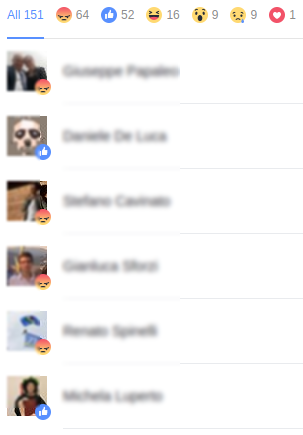
\includegraphics[width=.9\linewidth]{./img/sample2.png}
\caption{\label{fig:sample2}Detailed view of the users' reactions}
\end{figure}

\begin{figure}[htb]
\centering
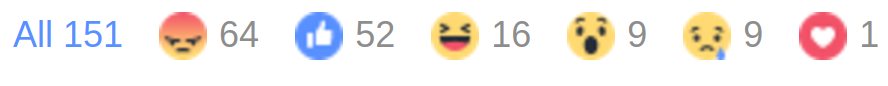
\includegraphics[width=.9\linewidth]{./img/sample3.png}
\caption{\label{fig:sample3}The reaction count vector. In this case the emotions are, from left to right, \texttt{ANGRY, LIKE, HAHA, WOW, SAD, LOVE.}}
\end{figure}

We selected four newspaper pages to scrape: a news agency (\texttt{AgenziaANSA}), one unbiased newspaper (\texttt{LaStampa}), a right-wing journal (\texttt{ilGiornale}) and a left-wing one (\texttt{ilManifesto}).

\subsection{Data}
\label{sec-2-2}

Table \ref{tab:sample-dataset} shows how the resulting dataset is structured: each headline is matched to a vector containing the raw counts of the users' reactions. Figure \ref{fig:sample2} shows an example of users' reactions and Figure \ref{fig:sample3} shows the total counts.

The present size of the dataset amounts to 479 news headlines. We are going to compute the entropy over the reaction count vectors.

\begin{table*}[htb]
\caption{\label{tab:sample-dataset}Sampe rows from the dataset}
\centering
\begin{tabular}{lrrrrrr}
text & LIKE & LOVE & ANGRY & HAHA & WOW & SAD\\
\hline
Le grandi tappe della Guerra fredda & 379 & 1 & 3 & 1 & 1 & 1\\
\#Fisco, case ecologiche ed e-bike & 393 & 4 & 3 & 11 & 1 & 1\\
\end{tabular}
\end{table*}

\subsection{Entropy}
\label{sec-2-3}

In this section we will be explaining what entropy is and why is it useful: we think that it is a concept that can be applied to many different problems and for this reason it is worth understanding it properly.

\begin{equation}
H(X)=\sum_{i}-P(i)log_{2}P(i)
\end{equation}

One one to think of entropy, is to interpret is as a measure of uncertainty or surprise: the more uncertain we are about something happening, or the more surprised we are, the higher the entropy. The graph in Figure \ref{fig:bentropy-plot} shows the relation between entropy and probability: entropy is high when two different outcomes have the same probability.

\begin{figure}[htb]
\centering
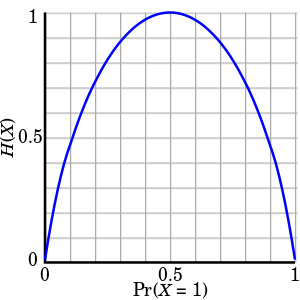
\includegraphics[width=.9\linewidth]{./img/bentropy_plot.png}
\caption{\label{fig:bentropy-plot}TODO Describe}
\end{figure}

It is possibile to think of entropy as a measure of skweness and its relation with kurtosis would be inversal:


Another way to interpret entropy is to think of it as a measure of impurity. Figure \ref{fig:classes-purity} represents two groups: the left group is much more impure than the right one and thus its entropy will be higher.

\begin{figure}[htb]
\centering
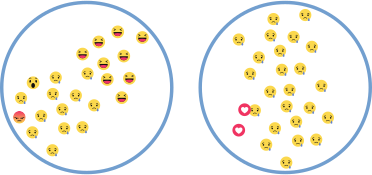
\includegraphics[width=.9\linewidth]{./img/classes.png}
\caption{\label{fig:classes-purity}Two groups representing two fictious sets of reactions to two posts.}
\end{figure}

\subsection{Using entropy as a proxy for annotations}
\label{sec-2-4}

In order to use entropy as a proxy for annotations, we need to define how it is related to controversy. From our definition of controversy and from our dataset, we can say that a headline is controversal when at least two emotion classes show high counts; the following (fictious) example makes this clear:

\begin{table}[htb]
\caption{\label{tab:example-controvery}A fictious example of a controversal headline}
\centering
\begin{tabular}{lrr}
text & WOW & SAD\\
\hline
Clinton has an 85\% chance to win & 500 & 350\\
\end{tabular}
\end{table}

The lower the entropy, the more skewed the distribution will be:


\begin{figure}[htb]
\centering
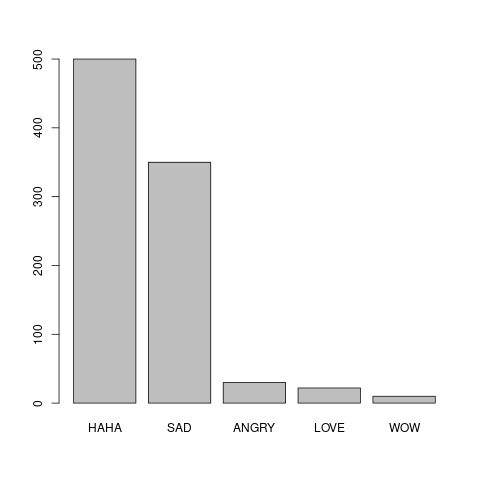
\includegraphics[width=.9\linewidth]{./img/a1barplot1.png}
\caption{\label{fig:bar-plot}TODO Describe}
\end{figure}

\subsection{Results}
\label{sec-2-5}

In order to evaluate the results we have to manually inspect the data. After sorting the headlines by decreasing entropy we get the followings:

[TODO ADD text]

\section{Discussion, Conclusion and Future Work}
\label{sec-3}


By manually inspecting the sorted dataset we found that the method produced good results. Unfortunately, we don't have any other metric other than human judjement.

The results obtained by using distant supervision methods should always be considered as \emph{silver data}: for this reason we plan to have human annotators reviewing the dataset; given the nature of the task, we plan to have at least two annotators working on the same data in order to compare how often they will agree.

We have to note that deciding how to use the signal in the data (reactions, in this case) is not obvious: for example, we decided to leave out the \texttt{LIKE} column when computing the entropy, because it lead to less interpretable data and an average lower entropy for all the headlnes. However, those users who use the \texttt{LIKE} reaction to express agreement with the content, will not use the \texttt{LOVE} reaction: this should mean that in general the positive reactions might always be lower than what they would have been if we had treated \texttt{LIKE} as a positive reaction.

Summarising, we proposed a method for finding controversal headlines on Facebook using entropy. By manually inspecting the results we found the method to be successfull.

For the next step we will be modeling the text in order to predict the entropy score automatically. Additionally, we will investigate how a news reporting on the same event is received by different audiences.

\section{Acknowledgments}
\label{sec-4}

We are thankful to the instructors and the students of the Methodology \& Statistics for Linguistic Reaserch Class (2017) of the University of Gronigen for the useful feedback provided.
% Emacs 25.2.1 (Org mode 8.2.10)
\end{document}
